%%
%% This is file `sample-manuscript.tex',
%% generated with the docstrip utility.
%%
%% The original source files were:
%%
%% samples.dtx  (with options: `all,proceedings,bibtex,manuscript')
%% 
%% IMPORTANT NOTICE:
%% 
%% For the copyright see the source file.
%% 
%% Any modified versions of this file must be renamed
%% with new filenames distinct from sample-manuscript.tex.
%% 
%% For distribution of the original source see the terms
%% for copying and modification in the file samples.dtx.
%% 
%% This generated file may be distributed as long as the
%% original source files, as listed above, are part of the
%% same distribution. (The sources need not necessarily be
%% in the same archive or directory.)
%%
%%
%% Commands for TeXCount
%TC:macro \cite [option:text,text]
%TC:macro \citep [option:text,text]
%TC:macro \citet [option:text,text]
%TC:envir table 0 1
%TC:envir table* 0 1
%TC:envir tabular [ignore] word
%TC:envir displaymath 0 word
%TC:envir math 0 word
%TC:envir comment 0 0
%%
%% The first command in your LaTeX source must be the \documentclass
%% command.
%%
%% For submission and review of your manuscript please change the
%% command to \documentclass[manuscript, screen, review]{acmart}.
%%
%% When submitting camera ready or to TAPS, please change the command
%% to \documentclass[sigconf]{acmart} or whichever template is required
%% for your publication.
%%
%%
\documentclass[manuscript,screen]{acmart}

% Core for drawing
\usepackage{tikz}
\usetikzlibrary{arrows.meta,positioning,shapes.geometric,fit}
% pgfplots (the plotting package on top of TikZ)
\usepackage{pgfplots}
\pgfplotsset{compat=1.18}

\usepackage{booktabs}
%%
%% \BibTeX command to typeset BibTeX logo in the docs
\AtBeginDocument{%
  \providecommand\BibTeX{{%
    Bib\TeX}}}

%% Rights management information.  This information is sent to you
%% when you complete the rights form.  These commands have SAMPLE
%% values in them; it is your responsibility as an author to replace
%% the commands and values with those provided to you when you
%% complete the rights form.
\setcopyright{none}

%%
%% end of the preamble, start of the body of the document source.
\begin{document}

%%
%% The "title" command has an optional parameter,
%% allowing the author to define a "short title" to be used in page headers.
\title{Evaluation of Intermediate Steps in Retrieval Augmented Generation}

\author{Aram Aytekin}
\affiliation{%
  \institution{Universität Kassel}
  \country{Germany}}
\email{uk097201@student.uni-kassel.de}

\author{Moritz Dietrich}
\affiliation{%
  \institution{Universität Kassel}
  \country{Germany}}
\email{uk097299@student.uni-kassel.de}

\author{Maximilian Bennedik}
\affiliation{%
  \institution{Universität Kassel}
  \country{Germany}}
\email{uk095879@student.uni-kassel.de}

\author{Domenic Bremmer}
\affiliation{%
  \institution{Universität Kassel}
  \country{Germany}}
\email{uk095482@student.uni-kassel.de}


%%
%% By default, the full list of authors will be used in the page
%% headers. Often, this list is too long, and will overlap
%% other information printed in the page headers. This command allows
%% the author to define a more concise list
%% of authors' names for this purpose.
\renewcommand{\shortauthors}{A. Aytekin, M. Dietrich, M. Bennedik, D. Bremmer}

%%
%% The abstract is a short summary of the work to be presented in the
%% article.
\begin{abstract}
This work investigates the research question: Does a RAG pipeline that expands the initial prompt into an LLM-generated query pool produce answers that humans prefer (on correctness, conciseness, and relevance) over a baseline that directly queries Elasticsearch once? To explore this, we implement two retrieval-augmented generation (RAG) pipelines that operate exclusively on search engine result page (SERP) snippets, which are often incomplete and inconsistent. The baseline pipeline (P1) retrieves snippets from a single query and directly conditions an LLM on this evidence. The advanced pipeline (P4), in contrast, employs LLM-based query expansion to generate a pool of reformulated queries, filters the resulting snippets, and integrates them for answer inference. Human evaluation indicates that P4 produces answers that are slightly more coherent, contextually appropriate, and preferred overall, though the improvements remain moderate. However, these gains come at the cost of significantly longer execution time, highlighting a trade-off between answer quality and system efficiency. These findings demonstrate the potential of query-expansion-based RAG pipelines for enhancing answer quality from fragmented snippet collections, while also pointing to open challenges in efficiency, evidence integration, and domain adaptation.
\end{abstract}

%%
%% The code below is generated by the tool at http://dl.acm.org/ccs.cfm.
%% Please copy and paste the code instead of the example below.
%%
\begin{CCSXML}
\begin{CCSXML}
<ccs2012>
   <concept>
       <concept_id>10002951.10003317.10003338</concept_id>
       <concept_desc>Information systems~Retrieval models and ranking</concept_desc>
       <concept_significance>500</concept_significance>
       </concept>
   <concept>
       <concept_id>10002951.10003317.10003359</concept_id>
       <concept_desc>Information systems~Evaluation of retrieval results</concept_desc>
       <concept_significance>500</concept_significance>
       </concept>
   <concept>
       <concept_id>10010147.10010178.10010179</concept_id>
       <concept_desc>Computing methodologies~Natural language processing</concept_desc>
       <concept_significance>300</concept_significance>
       </concept>
 </ccs2012>
\end{CCSXML}

\ccsdesc[500]{Information systems~Retrieval models and ranking}
\ccsdesc[500]{Information systems~Evaluation of retrieval results}
\ccsdesc[300]{Computing methodologies~Natural language processing}

%%
%% Keywords. The author(s) should pick words that accurately describe
%% the work being presented. Separate the keywords with commas.
\keywords{RAG, Summary, Pooling, Query, LLM, Pipeline}

%\received{20 February 2007}
%\received[revised]{12 March 2009}
%\received[accepted]{5 June 2009}

%%
%% This command processes the author and affiliation and title
%% information and builds the first part of the formatted document.
\maketitle

\section{Introduction}
\label{sec:introduction}

Large language models (LLMs) and retrieval-augmented generation (RAG) have transformed information retrieval and answer generation. Yet, in many real-world scenarios such as search engines, only fragmented snippets from search engine result pages (SERPs) are available rather than full documents. These snippets are incomplete and heterogeneous, making coherent answer generation challenging but practically important.

A key issue lies in query handling. Single-query retrieval often misses relevant evidence, while LLM-driven query expansion promises broader coverage and more diverse evidence. Whether such query pooling improves answer quality from SERP snippets remains unclear. Our study therefore asks:  
\emph{Does a RAG pipeline with LLM-based query expansion produce answers that humans prefer—on correctness, conciseness, and relevance—over a baseline with a single direct query?}

To address this, we compare two pipelines operating solely on SERP snippets. The baseline (P1) issues one query and generates answers directly. The advanced pipeline (P4) expands the query into a pool, retrieves and filters additional snippets, and conditions generation on this evidence. We evaluate both through human preference judgments and runtime cost measurements. Results show that P4 yields slightly more coherent answers but at substantially higher cost, revealing a trade-off between quality and efficiency in query-expansion-based RAG pipelines.

\section{Background \& Related Work}
\label{sec:background}

	\subsection{Retrieval Augmented Generation}
	\label{subsec:retrieval-augmented-generation}
	Retrieval-Augmented Generation (RAG) combines LLMs with external retrieval to produce factually grounded answers \cite{izacard-grave-2021-leveraging,NEURIPS2020_6b493230}. By conditioning responses on retrieved documents, RAG mitigates hallucinations and improves factuality in tasks such as open-domain QA and summarization \cite{karpukhin-etal-2020-dense,guu2020realmretrievalaugmentedlanguagemodel}. Unlike most prior work assuming access to full documents, our study targets fragmented SERP snippets, which introduces challenges for coherent answer generation.
	
	\subsection{Query Expansion vs. Single-Query Baselines}
	\label{subsec:query-expansion-vs-baseline}
	Single-query retrieval is efficient but risks missing evidence. Query expansion addresses this by generating variant queries, improving coverage but also adding cost and potential noise \cite{nogueira2020passagererankingbert,wang-etal-2023-query2doc}. Our baseline (P1) represents the single-query setup, while P4 applies LLM-driven expansion within RAG, enabling systematic cost–quality comparison.
	
	\subsection{Human Preference Evaluation}
	\label{subsec:human-preference-eval}
	Automatic metrics such as BLEU, ROUGE, or BERTScore often fail to capture open-ended answer quality \cite{post-2018-call,lin-2004-rouge,zhang2020bertscoreevaluatingtextgeneration}. Human evaluation remains the gold standard, typically via pairwise preference judgments \cite{bai2022traininghelpfulharmlessassistant,stiennon2022learningsummarizehumanfeedback}. Crowdsourcing offers scalable evaluation for RAG systems \cite{Gienapp_2025}. In our study, we compare P1 vs.~P4 answers along correctness, conciseness, and relevance, providing direct evidence for the impact of query pooling on perceived quality.

\section{Methods}

	\subsection{Pipelines}
	\label{subsec:pipelines}
	
	In this project \cite{repo}, we compare two retrieval-augmented generation pipelines that
	differ in how they formulate and execute search queries before producing an
	LLM-based answer.
	
	\paragraph{Pipeline 1: Direct Retrieval and Answering.}
	In this baseline approach, the system directly takes the user’s input prompt
	and submits it as a query to the Elasticsearch retriever. The retriever returns the top-$k$ relevant text
	snippets, which are then provided to the LLM together with a
	strict system instruction: the model must formulate its answer \emph{only based
	on the retrieved snippets}. This ensures that the output is grounded in the
	search results without additional query expansion or prompt reformulation.
	
	\begin{figure}[H] % or [htbp]
		\centering
		\resizebox{\textwidth}{!}{%
		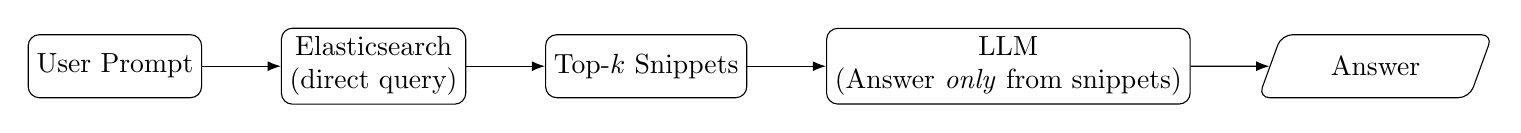
\begin{tikzpicture}[
		  node distance=7mm and 10mm, >=Latex,
		  box/.style={draw, rounded corners, align=center, minimum height=8mm, inner sep=3pt},
		  process/.style={box}, io/.style={box, trapezium, trapezium left angle=70, trapezium right angle=110}
		]
		\node[process] (p1_prompt) {User Prompt};
		\node[process, right=of p1_prompt] (p1_retr) {Elasticsearch\\(direct query)};
		\node[process, right=of p1_retr] (p1_snips) {Top-$k$ Snippets};
		\node[process, right=of p1_snips] (p1_llm) {LLM\\(Answer \emph{only} from snippets)};
		\node[io,      right=of p1_llm] (p1_out) {Answer};
		
		\draw[->] (p1_prompt) -- (p1_retr);
		\draw[->] (p1_retr) -- (p1_snips);
		\draw[->] (p1_snips) -- (p1_llm);
		\draw[->] (p1_llm) -- (p1_out);
		\end{tikzpicture}%
		}
		\caption{Pipeline~1 — direct retrieval from Elasticsearch and grounded answering from retrieved snippets.}
		\label{fig:pipeline1}
	\end{figure}
	
	\paragraph{Pipeline 4: Query Pool Expansion.}
	This enhanced approach adds an intermediate reasoning step before retrieval.
	The LLM is first asked to generate a \emph{query pool}, i.e.\ a set of
	reformulated or semantically related search queries derived from the original
	user prompt. These multiple queries are then executed against Elasticsearch,
	leading to a richer and more diverse set of retrieved snippets. The snippets
	are aggregated and passed to the LLM, which produces the final answer. By
	broadening the retrieval space, Pipeline~4 aims to increase coverage and
	relevance compared to the single-query baseline.
	
	\begin{figure}[H]
		\centering
		\resizebox{\textwidth}{!}{%
		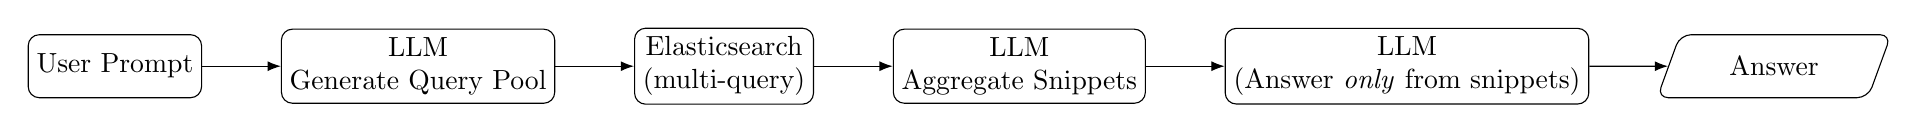
\begin{tikzpicture}[
		  node distance=7mm and 10mm, >=Latex,
		  box/.style={draw, rounded corners, align=center, minimum height=8mm, inner sep=3pt},
		  process/.style={box}, io/.style={box, trapezium, trapezium left angle=70, trapezium right angle=110}
		]
		\node[process] (p4_prompt) {User Prompt};
		\node[process, right=of p4_prompt] (p4_qpool) {LLM\\Generate Query Pool};
		\node[process, right=of p4_qpool] (p4_retr) {Elasticsearch\\(multi-query)};
		\node[process, right=of p4_retr] (p4_snips) {LLM\\Aggregate Snippets};
		\node[process, right=of p4_snips] (p4_llm) {LLM\\(Answer \emph{only} from snippets)};
		\node[io,      right=of p4_llm] (p4_out) {Answer};
		
		\draw[->] (p4_prompt) -- (p4_qpool);
		\draw[->] (p4_qpool) -- (p4_retr);
		\draw[->] (p4_retr) -- (p4_snips);
		\draw[->] (p4_snips) -- (p4_llm);
		\draw[->] (p4_llm) -- (p4_out);
		\end{tikzpicture}%
		}
		\caption{Pipeline~4 — LLM-generated query pool, multi-query retrieval, snippet aggregation, and grounded answering.}
		\label{fig:pipeline4}
	\end{figure}



	\subsection{Retrieval configuration}
	\label{subsec:retrieval-config}
	
	\paragraph{Data.}
	We retrieve over an Elasticsearch index built from the \emph{Archive Query Log (AQL-22)}~\citep{reimer:2023}, a corpus of archived search engine result pages (SERPs) containing historical queries and their snippet-level results (titles, snippets, target URLs). Crucially, because these SERPs are captured from the Internet Archive, the queries and their retrieved contexts are \emph{reproducible}; unlike commercial engines (e.g., Google) whose indices and ranking algorithms change over time, AQL provides a stable snapshot that makes our comparative analysis possible.
	
	\paragraph{Source retriever.}
	Our retriever queries the AQL-backed Elasticsearch index to collect snippet contexts that ground LLM answers. In \textbf{Pipeline~1}, the user prompt is issued as a single ES query; we take the top-$k$ snippets and pass them to the LLM with an instruction to answer \emph{only} from those snippets. In \textbf{Pipeline~4}, the LLM first generates a pool of reformulated queries; we execute each against the same index, merge and deduplicate the returned snippets, then feed the aggregated context to the LLM. Both pipelines operate on the identical index and use the same $k$ and filtering/cleanup steps to isolate the effect of the query strategy itself.
	
	\subsection{LLM Configuration}
	\label{subsec:llm-config}
	
	This subsection describes the configuration and prompting strategy used for the large language models (LLMs) in our pipelines. Each LLM instance operates with a specialized system prompt defining its role, objectives, and constraints. The general workflow across pipelines includes generating relevant queries, retrieving or aggregating context snippets, and producing answers grounded in those snippets.
	
	All LLM calls in this work are performed using the Helmholtz-Blablador API~\cite{blablador_api} with the model \texttt{"alias-large"}~\cite{qwen3_model}, also referred to as Qwen3-30B-A3B, optimized for information retrieval and question-answering tasks.
	
	The following sections detail the three main stages of LLM configuration: \textit{Query Pool Generation}, \textit{Snippet Aggregation}, and \textit{Answer Generation}. Specific pipelines may implement subsets of these stages or additional mechanisms.
	
		\paragraph{Query Pool Generation}
		\label{subsubsec:query-pool-generation}
		
		The system prompt guides the LLM in producing concise and meaningful search queries from a user's question by extracting core subjects, typically the most important nouns, entities, or concepts. This ensures that generated queries are focused on essential terms for downstream retrieval.
		
		\paragraph{Snippet Aggregation}
		\label{subsubsec:snippet-aggregation}
		
		After generating a query pool and retrieving candidate snippets, the LLM evaluates which snippets are relevant for answering the user's question. The model is instructed to retain any snippet that might provide useful information, including direct answers, relevant facts, supporting examples, or background context, and to exclude only unrelated content.
		
		\paragraph{Answer Generation}
		\label{subsubsec:answer-generation}
		
		In both Pipelines 1 and 4, the final step is to generate a concise answer strictly based on the selected context snippets. The system prompt instructs the LLM to provide clear, direct responses in no more than five sentences. Only information present in the snippets may be used; if the context lacks sufficient information, the model indicates that no answer is available.
	
	
	\subsection{Evaluation Protocol}
	\label{subsec:evaluation-protocol}
	
	We curated a set of 20 predefined user questions and executed each question on
	both systems: \textbf{Pipeline~1} (single direct query) and \textbf{Pipeline~4}
	(LLM-generated query pool). For each prompt, this produced two answers, one from
	each pipeline, generated under the same model and decoding settings.
	
	Human evaluation was conducted as a randomized, blind A/B test. For every
	prompt, the two answers were shown side-by-side with left/right positions
	randomized and the system identities hidden. Annotators followed the instructions
	in Section~\ref{subsec:annotator-remarks} (correctness as the primary criterion,
	then relevance and conciseness) and selected the preferred answer; a “No
	preference” option was available for ties.
	
	Our primary metric is the \emph{win rate}: the proportion of pairwise
	comparisons in which a pipeline’s answer was preferred, computed over
	non-tied votes. We report win rates per pipeline to compare overall preference.
	
	\subsection{Annotator Remarks}
	\label{subsec:annotator-remarks}
	
	Annotators compared two anonymous answers for each prompt and selected the
	better one according to three criteria. The primary dimension was
	\textbf{Correctness}, i.e., factual accuracy, avoidance of hallucinations, and
	consistency with the question. Secondary criteria were:
	
	\begin{itemize}
	  \item \textbf{Relevance}: whether the answer stays on-topic and addresses the prompt,
	  \item \textbf{Conciseness}: whether the response is complete yet compact, without unnecessary repetition.
	\end{itemize}
	
	The evaluation followed a strict priority order:
	\textbf{Correctness} $\rightarrow$ \textbf{Relevance} $\rightarrow$
	\textbf{Conciseness}. When criteria conflicted, annotators were instructed to
	prefer the answer that was more accurate and cautious, even if it was less
	polished. If both answers were equally good (or equally poor), annotators could
	indicate \emph{No preference}.
	
	After each vote, annotators briefly justified their decision with a short
	comment referring to the criteria (e.g., correctness of facts, conciseness, or
	topicality). Critical errors or omissions were expected to be highlighted in
	these remarks.
	
	Finally, annotators were reminded to judge only the written content itself:
	unsupported or incorrect claims were to be penalized more heavily than cautious
	ones, and external searches were not permitted. Stylistic polish or formatting
	was not to influence voting unless it directly affected clarity.

	
	\subsection{Hypotheses}
	\label{subsec:hypotheses}

	\paragraph{Rationale.}
	Pipeline~4 expands the initial prompt into an LLM-generated \emph{query pool}, increasing search coverage and expected recall of relevant snippets. Greater coverage should yield answers that are more accurate and on-topic, which, under our evaluation protocol, should translate into higher preference.
	
	\paragraph{Primary hypothesis.}
	\textbf{H\textsubscript{1}}~\label{hyp:H1}: Pipeline~4’s win rate exceeds $50\%$ over non-tied pairwise comparisons with Pipeline~1.\\
	\textbf{H\textsubscript{0}}~\label{hyp:H0}: Pipeline~4’s win rate is $\leq 50\%$.
	
	\paragraph{Note on latency.}
	Pipeline~4 may incur higher latency due to multi-query retrieval and increased LLM Overhead. We report latency distributions and mean times in the Results section, but latency is not part of the primary hypothesis test.


		
	\subsection{Cost Measurement}
	\label{subsec:cost-measure}

	\paragraph{What we measure.}
	To assess our secondary latency hypothesis (Section~\ref{subsec:hypotheses}), we record the
	\emph{LLM runtime} per prompt and pipeline: the \textbf{sum of time passed during all LLM
		calls} involved in producing an answer. For \textbf{Pipeline~1} this is the single
	answer-generation call. For \textbf{Pipeline~4} this includes the query-pool \emph{expansion}
	call, the filtering and aggregation call, and the final \emph{answer-generation} call. Measurements are taken at the application level and
	therefore include model inference time plus client–server overhead for the LLM service.
	
	\paragraph{Scope and aggregation.}
	We do not include Elasticsearch retrieval time or disk I/O—only LLM-invocation time. For each
	of the 20 questions and each pipeline, we compute the mean runtime across runs; we also report
	overall means and show per-question comparisons in the timing figures.
	
	\paragraph{Cost perspective.}
	\label{cost-perspective}
	Pipeline~1 is the lower bound, issuing exactly one LLM call. Pipeline~4 typically makes three (query expansion, snippet filtering/summarization, final answer), which raises latency and energy use. The filtering stage is the heaviest, since it ingests the largest raw snippet set; however, it often \emph{shrinks} the final context, partially offsetting token cost in the last generation step. In short: Pipeline~4 pays extra up front to reduce the payload of the final call.
	
	% (shortened a lot)
	Given that our model (\texttt{Qwen3-30B-A3B}) is an MoE (128 experts, 8 active), per-token compute is lower than dense models; prior work reports roughly 30–50\% savings, which helps amortize Pipeline~4’s additional calls~\cite{qwen3_model,yun2024inferenceoptimalmixtureofexpertlargelanguage}.

	
	\paragraph{Limitations.}
	Runtimes are not normalized by token counts and will co-vary with prompt/context length
	(Pipeline~4 typically supplies longer contexts due to multi-query aggregation). Transient
	network/provider variability may affect measurements. Because non-LLM retrieval stages are
	excluded, these numbers reflect the LLM portion of end-to-end latency and likely
	\emph{underestimate} total wall-clock differences between pipelines.

	
\section{Results}
\label{sec:results}
	
The win-rate figure (Fig.~\ref{fig:winrate-overall}) aggregates all non-tied
pairwise votes across the 20 prompts and shows a \emph{marginal} but significant average
advantage for \textbf{Pipeline~4} over \textbf{Pipeline~1}. As defined in
Section~\ref{subsec:evaluation-protocol}, “win rate” reflects the fraction of
comparisons in which a pipeline’s answer was preferred under our annotator
guidelines (Section~\ref{subsec:annotator-remarks}).

% Figure: Winrate
\begin{figure}[H]
\centering
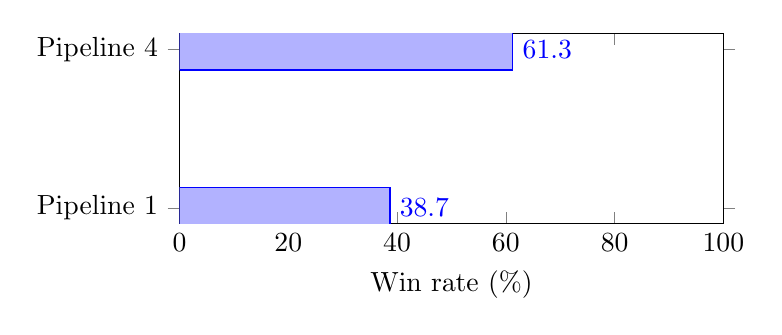
\begin{tikzpicture}
\begin{axis}[
  xbar,
  width=0.7\textwidth,
  height=4cm,
  xlabel={Win rate (\%)},
  xmin=0, xmax=100,
  symbolic y coords={Pipeline 1,Pipeline 4},
  ytick=data,
  nodes near coords,
  nodes near coords align={horizontal},
  bar width=15pt,
]
\addplot coordinates {(38.7,Pipeline 1) (61.3,Pipeline 4)};
\end{axis}
\end{tikzpicture}
\caption{Win rate comparison between Pipeline 1 and Pipeline 4.}
\label{fig:winrate-overall}
\end{figure}

\paragraph{Retrieval coverage limits.}
\label{retrieval-coverage-limits}
Not infrequently, Elasticsearch retrieved \emph{no accurate, on-topic snippets}
for a given prompt. In such cases, answers could not be fully grounded in the
provided context, compressing the attainable performance of either pipeline and
dampening any advantage from Pipeline~4’s broader query coverage.

\paragraph{Hallucinations on sensitive topics.}
We observed instances where the model answered \emph{regardless} of available
context, i.e., hallucinated content, particularly for highly sensitive topics
(e.g., COVID-19, climate change). This behavior violates the “answer only from
snippets” instruction and directly harms the \textbf{Correctness} criterion,
introducing variance in human preference that can overshadow small win-rate
differences.

\paragraph{Cost–latency perspective.}
Pipeline~4’s additional LLM calls for query-pool expansion (and occasional
aggregation) increase runtime and token usage roughly linearly with the extra
steps. Given the marginal improvement in win rate, the benefit may be
questionable when resources or latency budgets are tight.

% Figure: line plot of mean time per question (1..20)
\begin{figure}[H]
\centering
\begin{tikzpicture}
\begin{axis}[
  width=\textwidth,
  height=0.5\textheight,
  xlabel={Question (qid)},
  ylabel={Mean time (s)},
  xmin=1, xmax=20,
  xtick={1,...,20},
  ymajorgrids, xmajorgrids,
  legend style={at={(0.5,1.05)},anchor=south,legend columns=-1},
  enlarge x limits=0.02,
  unbounded coords=jump, % <-- prevents interpolation over NaNs
]

% Pipeline 1
\addplot+[
  mark=*,
  thick,
  color=blue,           % <-- force distinct color
  y filter/.code={%
    \edef\p{\thisrow{pipeline}}%
    \ifnum\pdfstrcmp{\p}{Pipeline 1}=0
      % keep value
    \else
      \def\pgfmathresult{nan}% hide non-matching rows
    \fi
  }
] table[
  x=qid, y=mean_time_seconds, col sep=comma
]{data/rag_time_long.csv};
\addlegendentry{Pipeline 1}

% Pipeline 4
\addplot+[
  mark=square*,
  thick,
  color=red,            % <-- force distinct color
  y filter/.code={%
    \edef\p{\thisrow{pipeline}}%
    \ifnum\pdfstrcmp{\p}{Pipeline 4}=0
      % keep value
    \else
      \def\pgfmathresult{nan}%
    \fi
  }
] table[
  x=qid, y=mean_time_seconds, col sep=comma
]{data/rag_time_long.csv};
\addlegendentry{Pipeline 4}

\end{axis}
\end{tikzpicture}
\caption{Mean LLM response times per question (s) for the two pipelines.}
\label{fig:time-per-question}
\end{figure}

\paragraph{Interpreting downward spikes.}
In Fig.~\ref{fig:time-per-question}, the sharp \emph{downward} spikes for
Pipeline~4 coincide with cases where Elasticsearch failed to retrieve
meaningful snippets. With little or no usable context, the expansion step
yields minimal material and the final answer call is short (often an abstention
or terse reply), reducing measured LLM runtime. These dips therefore reflect a
\emph{retrieval failure}, not an efficiency gain of the multi-query
pipeline.

\section{Conclusion}
\label{sec:conclusion}

We compared two RAG pipelines on 20 predefined prompts over the reproducible
Archive Query Log (AQL) index: a single-query baseline (Pipeline~1) and a
query-pool variant (Pipeline~4). In randomized, blind human voting, we observed
a \emph{modest} overall preference for Pipeline~4. 

\paragraph{Rationale.}
Pipeline~4 expands the initial prompt into an LLM-generated \emph{query pool}, 
increasing search coverage and expected recall of relevant snippets. Greater coverage 
should yield answers that are more accurate and on-topic, which, under our evaluation protocol, 
should translate into higher preference.

However, three factors temper this advantage: 
\newline(i) retrieval coverage gaps where Elasticsearch returned no meaningful snippets, limiting any pipeline’s ability to answer from context;  
\newline(ii) occasional hallucinations—especially on sensitive topics—where the model answered without sufficient grounding; and  
\newline(iii) higher LLM runtime for Pipeline~4 due to additional expansion/aggregation steps. Timing analysis shows
that apparent “fast” spikes for Pipeline~4 coincide with poor retrieval (short contexts), not genuine efficiency gains.

Overall, query-pool expansion helps when retrieval surfaces relevant evidence, and our results support \hyperref[hyp:H1]{H\textsubscript{1}}. 
While it cannot fully compensate for \hyperref[retrieval-coverage-limits]{weak recall} and may be undermined if grounding is not strictly followed, it provides consistent benefits in well-grounded settings. 
The \hyperref[fig:winrate-overall]{win-rate} gains remain modest, but the additional steps partly align with the rationale from the \hyperref[cost-perspective]{cost perspective}: paying more up front can sometimes shrink the final payload and improve answer focus. 
Still, in resource-constrained environments, the cost–quality trade-off requires careful consideration.


%%
%% The acknowledgments section is defined using the "acks" environment
%% (and NOT an unnumbered section). This ensures the proper
%% identification of the section in the article metadata, and the
%% consistent spelling of the heading.

%%
%% The next two lines define the bibliography style to be used, and
%% the bibliography file.
\bibliographystyle{ACM-Reference-Format}
\bibliography{cites}

\end{document}
\endinput
%%
%% End of file `sample-manuscript.tex'.
